\makeatletter
\def\input@path{{../../}}
\makeatother
\documentclass[../../main.tex]{subfiles}

\graphicspath{
	{../../img/}
	{../img/}
	{img/}
}

\begin{document}
	\subsection{Связь КрИ-2 и КрИ-1}
	
	Есть кривая:
	\[
	\begin{cases}
	x = x \left( t \right),\\
	y = y \left( t \right),\\
	\alpha \leq t \leq \beta
	\end{cases}
	\]
	
	\begin{center}
		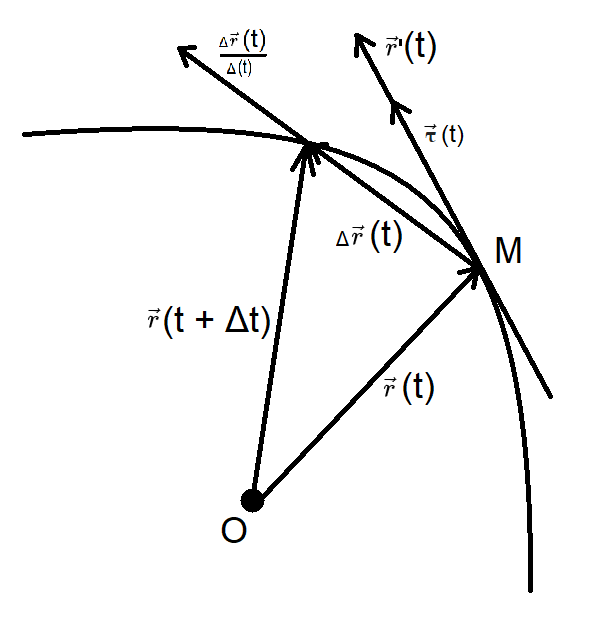
\includegraphics[scale = 0.8]{lec20_1.png}
	\end{center}
	
	Тогда:
	
	\[
	\overrightarrow{r} \left( t \right) = \left( x \left( t 
	\right),\, y \left( t \right) \right)
	\]
	
	\[
	\overrightarrow{\tau'} \left( t \right) = \left( x' \left( t 
	\right),\, y' \left( t \right) \right)
	\]
	
	Если $\Delta t \to 0$, то $\Delta\frac{r}{\Delta t}$
	$ \appr{\Delta t \to 0}
	\overrightarrow{r}(t)$
	
	Если $\Delta \overrightarrow{r} \to 0$, то $M$ приблизится к $N$
	и займет свое предельное положение.
	
	$\frac{\Delta r}{\Delta t}$ также меняется и займет свое предельное положение
	~--- касательный вектор кривой в точке $M$.
	
	\[
	\abs{\overrightarrow{r}} =
	\sqrt{\left( x'(t) \right)^2 + \left( y'(t) \right)^2}\,
	\]
	
	Если рассматривать $\overrightarrow{\tau} = 
	\frac{\overrightarrow{r}(t)}{\abs{\overrightarrow{r}}}$, то
	$\overrightarrow{\tau}$ ~--- касательный вектор,
	но $\abs{\overrightarrow{\tau}} = 1$, то есть:
	
	\[
	{\overrightarrow{r}} (\cos\alpha, \cos\beta),\,
	\]
	
	где $\alpha, \beta$ ~--- углы, образованные вектором $\overrightarrow{\tau}$
	или $\overrightarrow{r'}$ с положительными координатными полуосями
	$Ox$ и $Oy$	(соответствующие направляющие косинусы векторов
	$\overrightarrow{\tau}$	или $\overrightarrow{r'}$).
	
	Отсюда имеем:
	
	\[
	\overrightarrow{r'}(t) = \overrightarrow{\tau}(t)\abs{\overrightarrow{r'}(t)} 
	=
	(\abs{\overrightarrow{r'}(t)}\cos \alpha, \abs{\overrightarrow{r'}(t)}\cos 
	\beta)
	\implies\,
	\]
	
	\[
	\implies\, \begin{gathered}
	\overrightarrow{x'}(t) = \abs{\overrightarrow{r'}(t)}\cos \alpha\, \\
	\overrightarrow{y'}(t) = \abs{\overrightarrow{r'}(t)}\cos \beta\,
	\end{gathered}
	\]
	
	\[
	\begin{gathered}
	dx = \abs{\overrightarrow{r'}(t)} dt\cos \alpha\, \\
	dy = \abs{\overrightarrow{r'}(t)} dt\cos \beta\,
	\end{gathered}
	\]
	
	Если зафиксировать некоторое $t$, этому значению
	на кривой соответствует точка,
	которой соответствует значение параметра $S$:
	
	\[
	t \iff M(t) \iff S\, \text{~--- длина от точки}\, A\,.
	\]
	
	\[
	S = S(t) = \int\limits_{\alpha}^{t} \sqrt{\left( x'(t) \right)^2
	+ \left( y'(t) \right)^2}\, dt\,
	\]
	
	Отсюда (используя теорему Барроу) следует, что:
	
	\[
	S'(t) = \sqrt{\left( x'(t) \right)^2 + \left( y'(t) \right)^2}\, =
	\abs{\overrightarrow{r'}}\,
	\]
	
	Тогда:
	
	\[
	\abs{\overrightarrow{r'}}dt\, = \abs{\overrightarrow{s'}}dt\, = ds\,
	\]
	
	Получаем:
	
	\[
	\begin{gathered}
	dx = ds \cos \alpha\, = \cos \alpha\, ds\, \\
	dy = ds \cos \beta\, = \cos \beta\, ds\,
	\end{gathered}
	\]
	
	Поэтому:
	
	\begin{equation}
	\label{lec_20, num_1}
	\int\limits_{\overbow{AB}} P \left( x \left( t \right),\, y \left( t 
	\right) \right)\, dx + Q \left( x \left( t \right),\, y \left( t \right)
	\right)\, dy =
	\int\limits_{\overbow{AB}} \left( P \left(x, y \right)\, \cos \alpha\,
	+ Q \left(x, y \right)\, \cos \beta \right)ds
	\end{equation}
	
	Слева записан КрИ-2, справа КрИ-1 по одной и той же кривой.
	
	\begin{rem}
		Здесь в КРИ-2 направление на $\overbow{AB}$  ~---
		направление возрастания $t$,
		и косинусы соответствуют этому направлению.
	\end{rem}	
		
В случае КрИ-2 по произвольной кривой $\overbow{AB}$ имеем:

\[
\begin{gathered}
\int\limits_{\overbow{AB}} P \left(x, y, z \right)\, dx\,
+ Q \left(x, y, z \right)\, dy\, + R \left(x, y, z \right)\, dz\, = \\
= \int\limits_{\overbow{AB}} \left( P \left(x, y, z \right)\, \cos \alpha\,
+ Q \left(x, y, z \right)\, \cos \beta\, + R \left(x, y, z \right)\, \cos 
\gamma\, \right)ds,
\end{gathered}
\]
где $P, Q, R$ ~--- функции от $x, y, z$; $\cos \alpha, \cos \beta,
\cos \gamma$ ~--- направляющие косинусы касательного вектора
к $\overbow{AB}$.
	
	\begin{rem}
		Если прямая кусочно-гладкая, т.~е. состоит из конечного множества дуг,
		каждая из которых ~--- гладкая кривая, то разбиваем интеграл, используя
		свойство аддитивности (прямая не обязательно непрерывная).
	\end{rem}

\subsection{Формула Грина}

Пусть $D \subset \R^2$ ~--- некоторая область из $\R^2$, в которой
располагается замкнутая область $G \subset D$ с границей $L$.

Говорят, что на $L$ выбрано положительное направление,
если при движении в таком направлении область $G$ остается слева
(то есть против часовой стрелки).

\begin{center}
	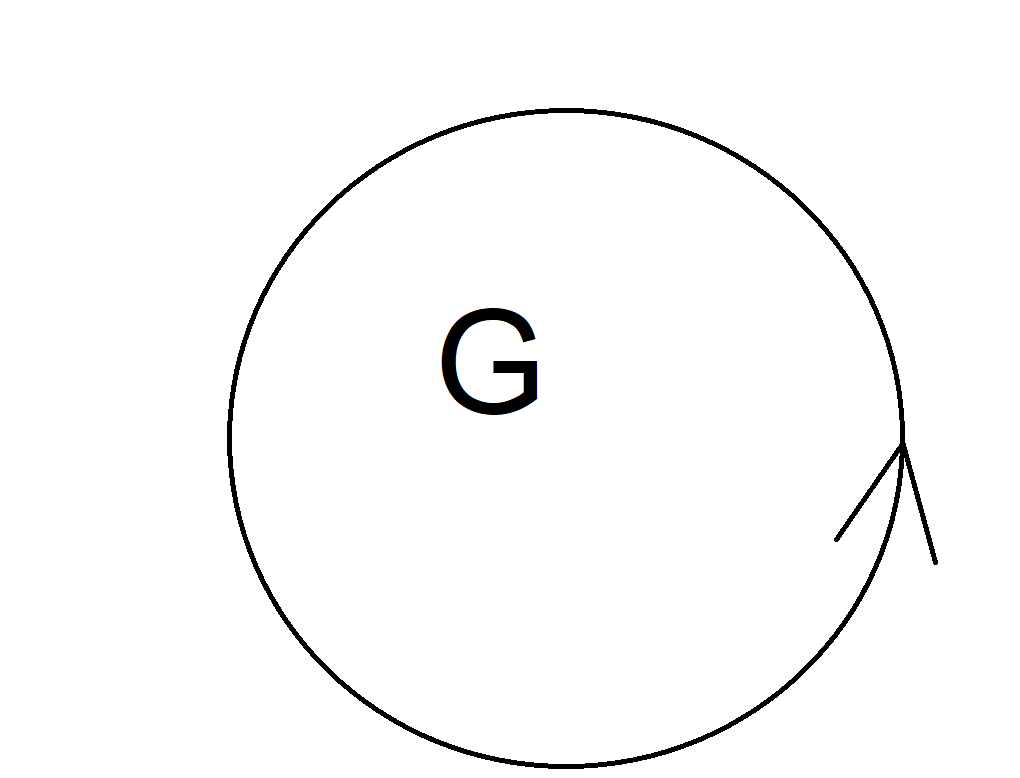
\includegraphics[scale = 0.4]{lec20_2.png}
\end{center}

\begin{thm}
	Если функции $P$ и $Q$ непрерывны и имеют непрерывные частные производные 
	$P'_y, Q'_x$, то:
	
	\begin{equation}
	\label{lec_20, num_2}
	\int\limits_{L} P \left( x, y \right)\, dx + Q \left( x, y \right)\,
	dy = \int\limits_{G}\int \left( G_x' \left(x, y \right)\,
	- P_y' \left(x, y \right)\, \right)\, dx\, dy\,
	\end{equation}
	
	где $L$ пробегает в положительном направлении.
	
	Слева находится КрИ-2, справа ~--- 2И.
\end{thm}

\begin{proof}
	Рассмотрим:
	
	\[
	- \int\limits_{G}\int P_y' \left(x, y \right)\, dx\, dy\,
	\]
	
	\begin{itemize}
		\item[а)] Область $G$ ограничена и представляется собой (AD, BC ~--- 
		вертикальные прямые):
		
		\begin{center}
			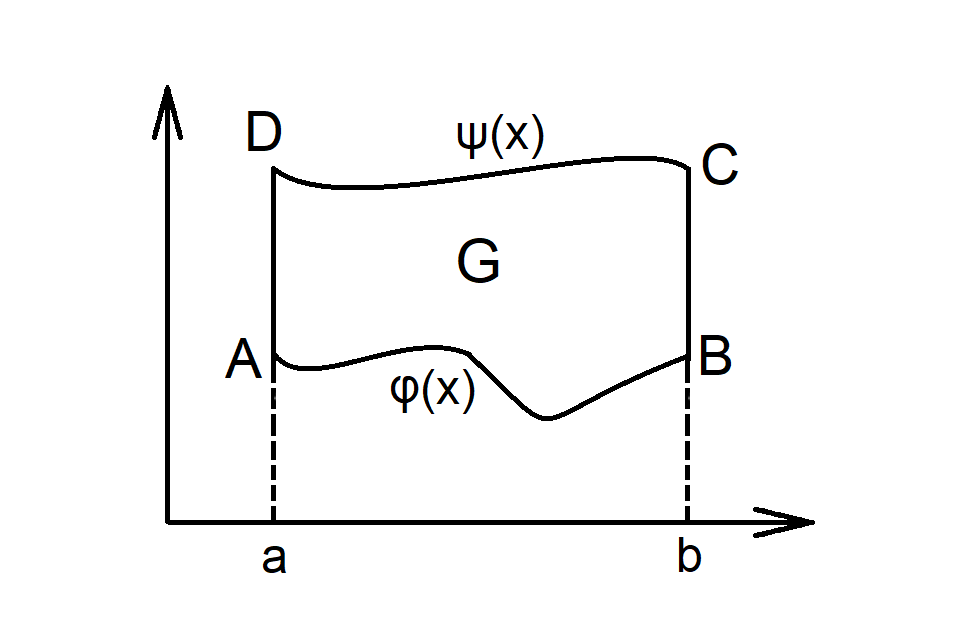
\includegraphics[scale = 0.8]{lec20_3.png}
		\end{center}
	
		Тогда:
		
		\[
		\begin{gathered}
			- \int\limits_{G}\int P_y' \left(x, y \right)\, dx\, dy\, =
			- \int\limits_{a}^{b}\, dx\, \int\limits_{\phi(x)}^{\psi(x)} P_y'
			\left(x, y \right)\, dy\, =
			- \int\limits_{a}^{b}\, \left(P \left(x, \psi(x) \right)\, -
			P \left(x, \phi(x) \right)\, \right) dx\, = \\
			= \int\limits_{b}^{a}\, P \left(x, \phi(x) \right)\, dx\, +
			\int\limits_{a}^{b}\, P \left(x, \psi(x) \right)\, dx\, = 
			\int\limits_{\overbow{AB}}\, P \left(x, y \right)\, dx\, +
			\int\limits_{\overbow{CD}}\, P \left(x, y \right)\, dx\, = \\
			= [\int\limits_{\overbow{BC}}\, P \left(x, y \right)\, dx\, = 0]\,
			= [\int\limits_{\overbow{DA}}\, P \left(x, y \right)\, dx\, = 0]\,	
			= \int\limits_{\overbow{AB}}\, P \left(x, y \right)\, dx\, +
			\int\limits_{\overbow{CD}}\, P \left(x, y \right)\, dx\, + \\
			+ \int\limits_{\overbow{BC}}\, P \left(x, y \right)\, dx\, +
			\int\limits_{\overbow{DA}}\, P \left(x, y \right)\, dx\, =
			\int\limits_{L}\, P \left(x, y \right)\, dx\,
		\end{gathered}
		\]
		
		То есть:
		
		\begin{equation}
		\label{lec_20, num_3}
		-\int\limits_{G}\int P_y' \left(x, y \right)\, dx\, dy\, = 
		\int\limits_{L}\, P \left(x, y \right)\, dx\,
		\end{equation}
		
		\item[б)] Если область $G$ имеет более сложную конфигурацию, ее разбивают
		на часть вида а) с помощью вертикальных отрезков и
		используют свойство аддитивности интегралов.
		
		Например:
		
		\begin{center}
			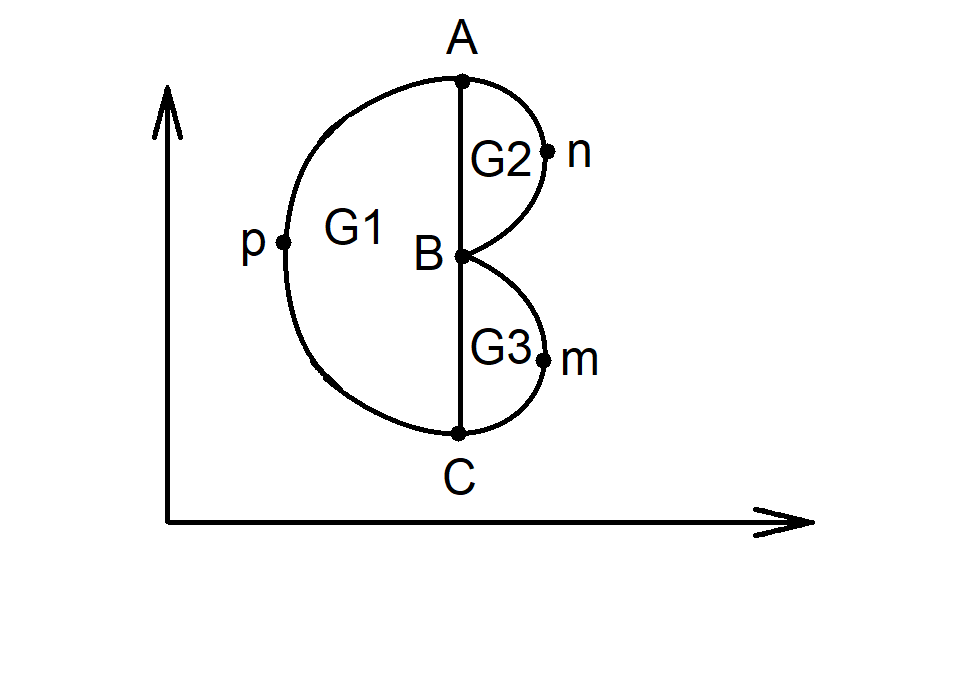
\includegraphics[scale = 0.8]{lec20_4.png}
		\end{center}
	
		\[
		\begin{gathered}
		\int\limits_{G}\int = \int\limits_{G_1}\int + \int\limits_{G_2}\int +
		\int\limits_{G_3}\int =
		\int\limits_{\overbow{ApC}} + \int\limits_{\overbow{CB}} +
		\int\limits_{\overbow{BA}} + \int\limits_{\overbow{BnA}} +
		\int\limits_{\overbow{AB}} + \int\limits_{\overbow{CmB}} +
		\int\limits_{\overbow{BC}} =
		\int\limits_{L}
		\end{gathered}
		\]		
	\end{itemize}

		Рассмотрим:
				
		\[
		\int\limits_{G}\int Q_x' \left(x, y \right)\, dx\, dy\,
		\]
		
		\begin{center}
			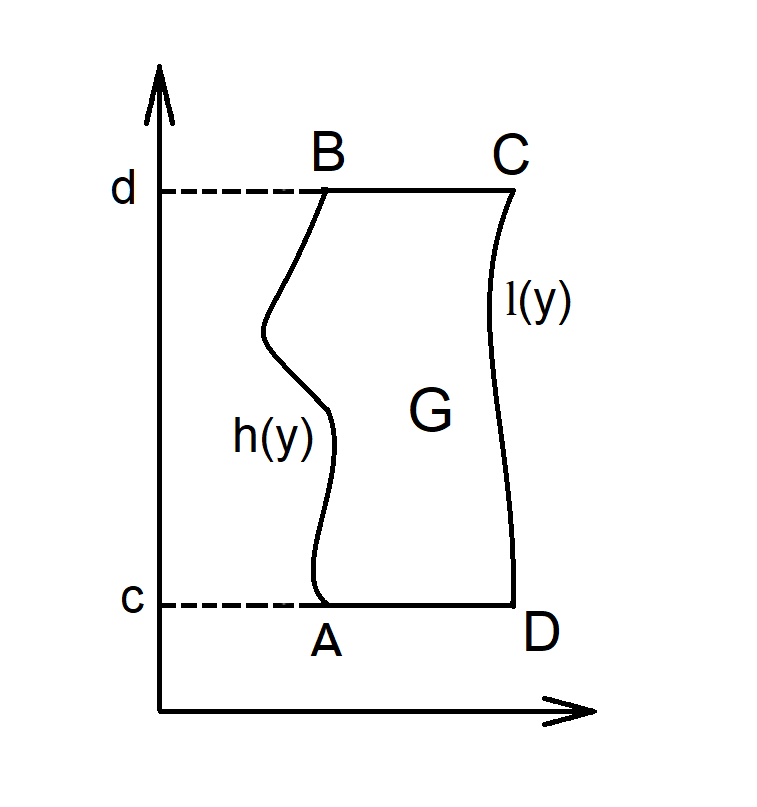
\includegraphics[scale = 0.6]{lec20_5.png}
		\end{center}
		
	\begin{itemize}
		\item[a)]
		\[
		\begin{gathered}
		\int\limits_{G}\int Q_x' \left(x, y \right)\, dx\, dy\, =
		\int\limits_{c}^{d}\, dy\, \int\limits_{h(x)}^{l(x)} Q_x'
		\left(x, y \right)\, dx\, =
		\int\limits_{c}^{d}\, \left(Q \left(l(x), y \right)\, -
		Q \left(h(x), y \right)\, \right) dy\, = \\
		= \int\limits_{c}^{d}\, Q \left(l(x), y \right)\, dy\, +
		\int\limits_{d}^{c}\, Q \left(h(x), y \right)\, dy\, =
		\int\limits_{c}^{d}\, Q \left(l(x), y \right)\, dy\, +
		\int\limits_{d}^{c}\, Q \left(h(x), y \right)\, dy\, = \\
		\int\limits_{\overbow{BC}}\, Q \left(l(x), y \right)\, dy\, +
		\int\limits_{\overbow{DA}}\, Q \left(h(x), y \right)\, dy\, =
		\int\limits_{\overbow{BC}}\, Q \left(l(x), y \right)\, dy\, +
		\int\limits_{\overbow{DA}}\, Q \left(h(x), y \right)\, dy\, + \\
		\int\limits_{\overbow{CD}}\, Q \left(l(x), y \right)\, dy\, +
		\int\limits_{\overbow{AB}}\, Q \left(h(x), y \right)\, dy\, =
		\int\limits_{L}\, Q \left(x, y \right)\, dy\,
		\end{gathered}
		\]
		
		\item[б)] Если $G$ ~--- область более сложной конфигурации, то ее
		разбивают на часть вида а) с помощью горизонтальных отрезков и
		используют свойство аддитивности интегралов.
	\end{itemize}

Получаем:

\begin{equation}
\label{lec_20, num_4}
\int\limits_{G}\int Q_x' \left(x, y \right)\, dx\, dy\, =
\int\limits_{L}\, Q \left(x, y \right)\, dy\,
\end{equation}

Сложив \eqref{lec_20, num_3} и \eqref{lec_20, num_4}, получим \eqref{lec_20, 
num_2}, используя свойство линейности КрИ.

\end{proof}

\subsection{Случай многосвязной области}

\begin{defn}
	Область $D$ называется односвязной, если любую замкнутую кривую $L \subset D$ 
	можно стянуть в точку, не выходя за пределы $D$.
\end{defn}

\begin{center}
	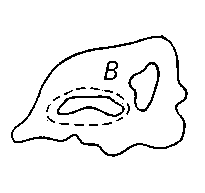
\includegraphics[scale = 1.5]{lec20_6.png}
\end{center}

Заштрихованная область является многосвязной.

Пусть в \eqref{lec_20, num_2} $G$ ~--- многосвязная область. Формула 
справедлива
и в этом случае. Такая $L$ пробегает в положительном направлении и
$L$ состоит из контуров $\l_1, \l_2, \l_3$.

\begin{center}
	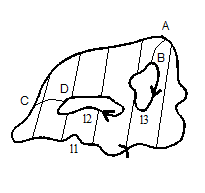
\includegraphics[scale = 1.5]{lec20_7.png}
\end{center}

Для доказательства соединим $\l_2, \l_3$ с $\l_1$ с помощью гладких
спрямляемых кривых.  Тогда область становится односвязной.

Граница состоит из $\overbow{AC} \cup \overbow{CB} \cup \l_3 \cup \overbow{DC} 
\cup \overbow{CA} \cup \overbow{AB} \cup \l_2 \cup \overbow{BA} = L$

При обходе $L$ в положительном направлении кривые $\overbow{AB}$ и 
$\overbow{CD}$ пробегают дважды в противоположных направлениях, поэтому сумма 
интегралов по этим кривым дает $0$.

То есть в КрИ-2 слева можно учитывать интегралы только по $\l_1, \l_2, \l_3$.
В 2И справа величина интеграла не измняется, так как кривые имеют нулевую 
площадь.

\begin{example}
	Вычислить $\displaystyle\int\limits_{\tiny{\overbow{AB}}} x^2 \cos y\, dx
	- \frac{x^3}{3}	\sin y\, dy,\  
	\text{по}\, \overbow{AB}:
	y = 3x - x^2$
	
	\begin{center}
		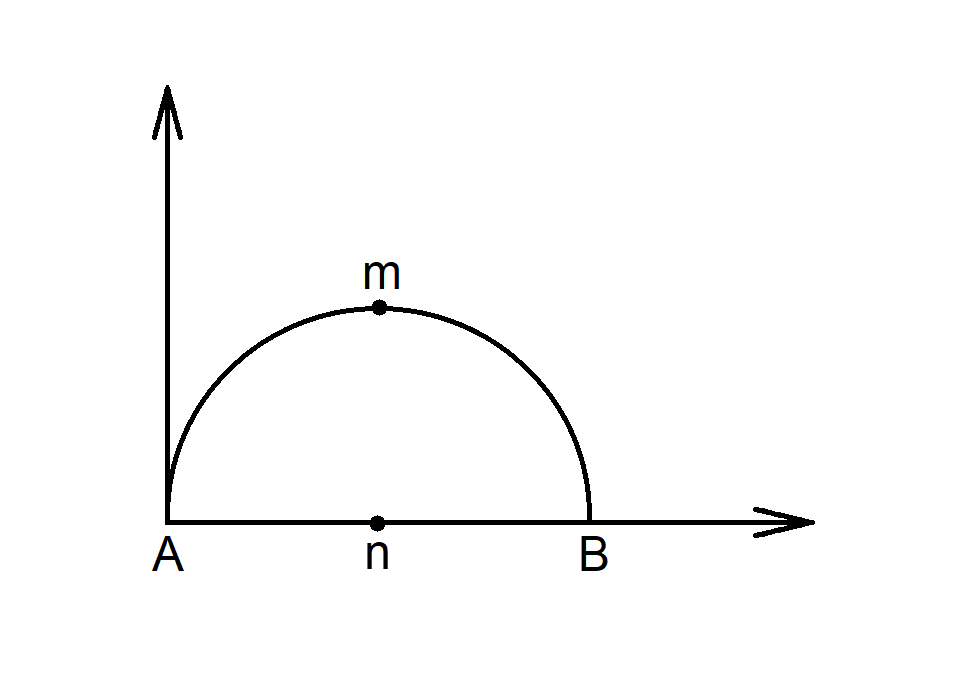
\includegraphics[scale = 0.5]{lec20_8.png}
	\end{center}

	Точки пересечения с осями: $A(0, 0), B(3, 0)$.
	
	\[
	\begin{gathered}
	\int\limits_{\tiny{\overbow{AB} \cup \overbow{BA}}} x^2 \cos y\, dx
	- \frac{x^3}{3}	\sin y\, dy,\ =
	\left[ \text{формула Грина} \right] =
	\int \limits_{\tiny{\overbow{AB}}}\int\, 0\, dx\, dy\,
	\implies
	\int\limits_{\tiny{\overbow{AB}}} =
	\int\limits_{\tiny{\overbow{AnB}}} = \\
	= \int\limits_{\tiny{\overbow{AnB}}} x^2 \cos y\, dx
	- \frac{x^3}{3}	\sin y\, dy,\ =	
	\left[ 
		\begin{gathered}
		\overbow{AnB}\, =\, 0\, \\
		0\, \leq\, x\, \leq\, 3\,
		\end{gathered}
	\right] =
	\int\limits_{0}^{3}\, x^2\, dx = 9
	\end{gathered}
	\]
\end{example}

\subsection{Вычисление площади с помощью КрИ}

Пусть требуется вычислить площадь области с границей $L$.

Если взять $P(x, y)$ и $Q(x, y)$ такие, что:

\[
Q_x'(x, y)\, - P_y'(x, y)\, = 1,\, \forall\, (x, y)\, \in G,\, \text{то}
\]

\[
\int\limits_{L} P\, dx\, + Q\, dy\, = \int\limits_{G}\int\, dx\, dy\,
= S = mes G
\]

Например:
	\begin{itemize}
		\item[a)] $ P(x, y)\, = 0\, Q(x, y)\, = x $
		\item[б)] $ P(x, y)\, = -y\, Q(x, y)\, = 0 $
		\item[в)] $ P(x, y)\, = -\frac{y}{2}\, Q(x, y)\, = \frac{x}{2} $
	\end{itemize}

\[
S = \int\limits_{L}\, x\, dy\, =
- \int\limits_{L}\, y\, dx\, =
\frac{1}{2}\, \int\limits_{L}\, x\, dy\, - y\, dx\,
\]

\begin{example}
	$\frac{x^2}{a^2}\, +\, \frac{y^2}{b^2}\, =\, 1$ ~--- уравнение $L$.
	
	\[
	\begin{gathered}
		S\, =\, \frac{1}{2}\int\limits_{L}\, x\, dy\, - y\, dx\, = 
		\left[
			\begin{gathered}
				x = a\, \cos t\, \\
				y = b \sin t\, \\
				0\, \leq\, t\, \leq\, 2x\,
			\end{gathered}
		\right] =
		\frac{1}{2}\, \int\limits_{0}^{2\pi}\, \left( a \cos t\, b \cos t\, +\,
		b \sin t\, a \cos t\, \right)\, dt\, = \\
		= \frac{ab}{2}\, \int\limits_{0}^{2\pi}\, dt\, =
		\pi ab
	\end{gathered}
	\]
\end{example}

\end{document}
